\documentclass{article}

\title{Math 3010 Midterm 1 "Cheat Sheet"}
\author{Lincoln Sand}

\usepackage{amsfonts}
\usepackage{graphicx}
\usepackage{amssymb}
\usepackage{amsmath}
\usepackage{listings}
\usepackage{hyperref}


\DeclareMathOperator{\sech}{sech}
\newcommand{\NN}{\mathbb{N}}
\newcommand{\RR}{\mathbb{R}}
\newcommand{\QQ}{\mathbb{Q}}
\newcommand{\ZZ}{\mathbb{Z}}
\newcommand{\dV}{\;\mathrm{d}V}
\newcommand{\dA}{\;\mathrm{d}A}
\newcommand{\dx}{\;\mathrm{d}x}
\newcommand{\dy}{\;\mathrm{d}y}
\newcommand{\dz}{\;\mathrm{d}z}
\newcommand{\cA}{\mathcal{A}}
\newcommand{\Bb}{\mathcal{B}}
\newcommand{\Ww}{\mathcal{W}}
\newcommand{\Dd}{\mathcal{D}}
\newcommand{\Ss}{\mathcal{S}}
\newcommand{\Ee}{\mathcal{E}}
\DeclareMathOperator{\im}{im}

\tolerance=1
\emergencystretch=\maxdimen
\hyphenpenalty=10000
\hbadness=10000

\setlength\parindent{10pt}

\begin{document}

Math 3010 Midterm 1 "Cheat Sheet"

Lincoln Sand

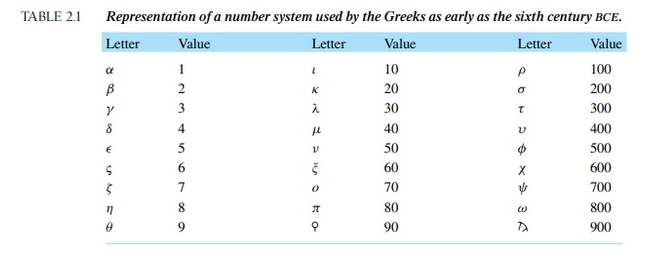
\includegraphics[width=\linewidth]{greek_numbers}

- Historical Data:

* Thales: 625 - 547 BC; Miletus; Advocated the deductive method. First man to have theorem named after him.

* Pythagoras: 580 - 497 BC; Croton; Explained musical harmony in terms of whole number ratios. Found some lengths are irrational.

* Zeno: 490 - 425 BC; Elia; Pupil of Parmenides. Proposed paradoxes involving infinity.

* Eudoxus: 400 - 347 BC; Cnidus; Devoloped theories of proportion and exhaustion.

* Aristotle: 384 - 322 BC; Athens; Advocated use of definitions/axioms/proofs in math and syllogism logic.

* Diophantus: 210 - 260 AD; Alexandria; Devloped algebraic notation and studied equations with integer unknowns.

* Archimedes: 287 - 212 BC; Syracuse; Discovered theorems using mechanical intuition with proofs.

* Euclid: 330 - 270 BC; Alexandria; His books set the standard for math rigor until 19th century.

* Plato: 427 - 346 BC; Athens; Theorems require sound definitions and proofs. The line and circle are pure.

* Hippocractes: 460 - 300 BC; Chios; Sophist philosopher, criticized fuzzy thinking. Squared the lune.

* Parmenides: 515 - 440 BC; Elia; Sophist, founded a school, "Whatever is is, and whatever is not cannot be".

* Chrysippus: 280 - 226 BC; Athens; Stoic philosopher, developed modern norations of evaluation of compound logic statements.

- Delian problems: Square the circle; Double the cube; Trisect an angle.

- Sum of geometric series:

\[S = \frac{a(1 - r^n)}{1-r}\]

If, $|r| < 1$, then it converges to:

\[S = \frac{a}{1-r}\]

- Euclidean GCD algorithm/diophantine example:

Find $x, y \in \ZZ$ such that $gcd(198, 168) = 198x + 168y$.

\[198 = 1 \cdot 168 + 30; 168 = 5 \cdot 30 + 18; 30 = 1 \cdot 18 + 12;\]
\[18 = 1 \cdot 12 + 6; 12 = 2 \cdot 6 + 0\]
So, $gcd(198, 168) = 6$.

\[6 = 18 - 12 = 18 - (30 - 18) = 2 \cdot 18 - 30 = 2 \cdot (168 - 5 \cdot 30) - 30\]
\[= 2 \cdot 168 - 11 \cdot 30 = 2 \cdot 168 - 11 \cdot (198 - 168) = 13 \cdot 168 - 11 \cdot 198\]
So, $x = -11, y = 13$.

- Five platonic solids:

Triangles: Three at a vertex, four at a vertex, five at a vertex.

Squares: Three at a vertex.

Pentagons: Three at a vertex.

Higher polygons: Can't form a vertex because interior angle is too large.

- Pell's equation:

\[x^2 - Ny^2 = 1, N \in \ZZ, N > 0\]

1) Find continued fraction for $\sqrt{N}$

2) Approximate the expansion as the convergent $\frac{h_i}{q_i}$

3) $(x, y)$ corresponds to a $(h_i, q_i)$

4) Check for fundamental solution. $(x_1, y_1)$ is the smallest non-trivial solution
and is called the fundamental solution.

\[x_{k+1} = x_1 x_k + N y_1 y_k\]
\[y_{k+1} = x_1 y_k + y_1 x_k\]
for $k \geq 1$.

- Example of method of false position:

We want to solve $x + \frac{x}{4} = 15$

Guess $x = 4$.

$x + \frac{4}{4} = 5$

This is off by 3, so guess $4 \cdot 3 = 12$.

$12 + \frac{12}{4} = 15$.

- Babylonian "divide and average" algorithm:

1) Start with initial guess $x_0$

2) Iterative step:

\[x_{n+1} = \frac{1}{2}\left(x_n + \frac{N}{x_n}\right)\]

3) Repeat the iterative step to desired accuracy.


\end{document}
